\documentclass[11pt,a4paper]{article}
%\usepackage[toc,page]{appendix}
\usepackage{graphicx}
\usepackage[a4paper]{geometry}
\usepackage{xcolor}
\usepackage{fancyhdr}
\usepackage{float}
\usepackage{setspace}
\usepackage[absolute]{textpos}
\usepackage{epstopdf}
%\usepackage[]{mcode} 	% To include matlab code
\usepackage{capt-of}
\usepackage{enumerate}
\usepackage{lastpage}
\usepackage{booktabs}
\usepackage{longtable}
\usepackage{array}
\renewcommand{\arraystretch}{1.5}

\usepackage[english]{babel}
\usepackage[utf8]{inputenc}
\usepackage{amsmath}
\usepackage{amsfonts}
\usepackage{graphicx}
\usepackage[colorinlistoftodos]{todonotes}
\usepackage{algorithm}
\usepackage{algpseudocode}
\usepackage{caption}
\usepackage{amsmath}
\usepackage{algorithm}
%\usepackage[noend]{algpseudocode}
\makeatletter
\def\BState{\State\hskip-\ALG@thistlm}
\makeatother

\usepackage{amsmath}
\usepackage{amsfonts}
\usepackage{amssymb}
\usepackage{eurosym}

%Tables
\usepackage{multirow}

% Header
\setlength{\headheight}{30pt}
\newgeometry{top=2.5cm, bottom = 1.5cm, left=2cm, right=2cm}
\pagestyle{fancy} 
\lhead{\includegraphics[height=0.8cm]{figures/{tue_logo}.png}}
%\lfoot{Group 4 - ``CASE"-HENK}
\cfoot{~}
\rfoot{Page \thepage ~of \pageref{LastPage}}

\usepackage{cleveref}
% Change cleveref reference eq. to equation same for figure
\crefname{equation}{equation}{equations}
\crefname{figure}{figure}{figures}
\crefname{table}{table}{tables}

% Change Section numbering to Problem 1
%\renewcommand{\thesection}{Problem \arabic{section}.}

\begin{document}
%\begin{titlepage}
%\vspace*{100pt}
%\begin{figure}
%\centering
%\includegraphics[width=0.5\textwidth]{figures/TUelogozondertekst}
%\end{figure}
%\begin{center}
%{ \huge \bfseries 4AT100 Automotive Systems Engineering Project\\[0.4cm] }
%\textsc{\Large Concept Project Plan}\\[0.5cm]
%
%\end{center}
%
%\vfill
%
%\renewcommand{\arraystretch}{1}
%
%\begin{flushleft} \large
%\begin{tabular}{l}
%Project Coordinators:\\
%Dr.Ir. A. van de Mortel-Fronczak (Asia) \\
%Dr.Ir. I. Barosan (Ion) \\
%\end{tabular}
%\end{flushleft}
%
%\begin{flushleft} \large
%\begin{tabular}{l l l l}
%Tutor: & & & \\
%L. Kefalidis (Lazaros) & & & \\
%& & & \\
%Authors:\hspace{30mm} 	& \hspace{35mm}	& \hspace{55mm} 	    		& 			\\
%S. Forno (Simone) 		& ​0978942		& T. de Mor\'ee (Tim)			& 0944052 	\\
%R.M.A. Goris (Rob) 		& 0808822		& T.M.A. van de Wiel (Thijs)	​& 0824530 	\\
%B.S. Haarsma (Bouke) 	& 0751757​		& H. Wils (Hielke) 				& 0807014 	\\
%\end{tabular}
%\end{flushleft}
%
%\begin{flushleft} \large
%\begin{tabular}{l}
%MSc. Programme Automotive Technology \\
%Eindhoven University of Technology \\
%\end{tabular}
%\end{flushleft}
%
%\begin{flushleft} \large
%\begin{tabular}{l}
%\today \hspace{8.4cm} Group 4 ``CASE"-HENK \\
%\end{tabular}
%\end{flushleft}
%
%\renewcommand{\arraystretch}{1.5}
%
%\end{titlepage}

\newgeometry{top=2.5cm, bottom = 3cm, left=2cm, right=2cm}

%\newpage
%
%\setcounter{tocdepth}{2}
%
%\tableofcontents
%\newpage


%------------------------------------------------

\section{Comparing Gmapping with Graph-Slam localization methods} \label{sec:comp}

According to the document $plan.xls$, to compare different localization methods a new $Graph-based$ one is introduced, using the ROS package [1]. Graph based Slam methods use a different mathematical model than for example $GMapping$, which uses Particle filter to calculate the robot posterior. According to [2] a graph-based SLAM algorithm represents the map by means of graphs. In this case, each node represents a pose of the robot along its trajectory and a set of sensor measurements. These are connected by arcs which represent the motion between successive poses. For each node, the map is computed by finding the spatial configuration of the nodes which are consistent with constraints from the arcs. In a nutshell, a graph-based approach is an optimization approach. \\
The way we proceed to compare the methods is depicted in Figure \ref{fig:schema}: we map the WZL environment first with $GMapping$ and then with $Karto-slam$. Even if the two approaches uses similar parameters for the filter, those are not required to be the same. Infact, as seen in Figure  \ref{fig:schema}, each built map is given as input to two different localizers, hence the input is always the same for both methods. We are satisfied with the $mapping$ process as soon as the map does not present the issues of [3]. Parameters used for $GMapping$ and $Karto-slam$ are found in Section \ref{sec:par}. The pose of the robot (localizers) is calculated using $Amcl$ and $Graph-localizer$, the latter provided by the ROS package [1].

\begin{figure}[h]
    \centering
    \begin{minipage}{.5\textwidth}
        \centering
        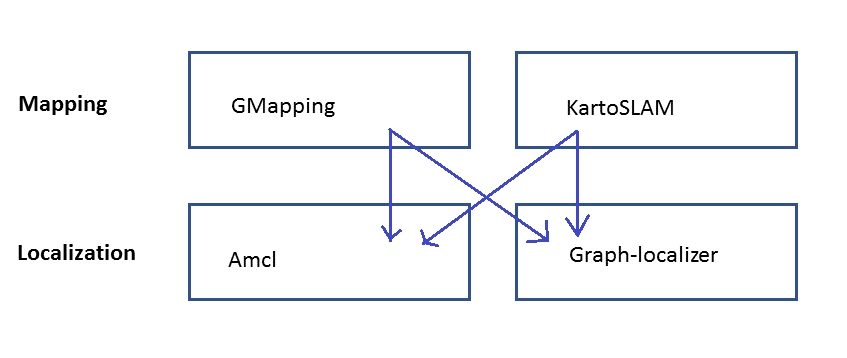
\includegraphics[width=0.9\linewidth, height=0.15\textheight]{figures/schema}
        \caption{Approach in comparing Amcl and Graph-based localization from different mappers. Each map is the single input for both the localizers. In this way it is possible to compare the robot poses under the same conditions}
        \label{fig:schema}
    \end{minipage}%
    \begin{minipage}{0.5\textwidth}
        \centering
        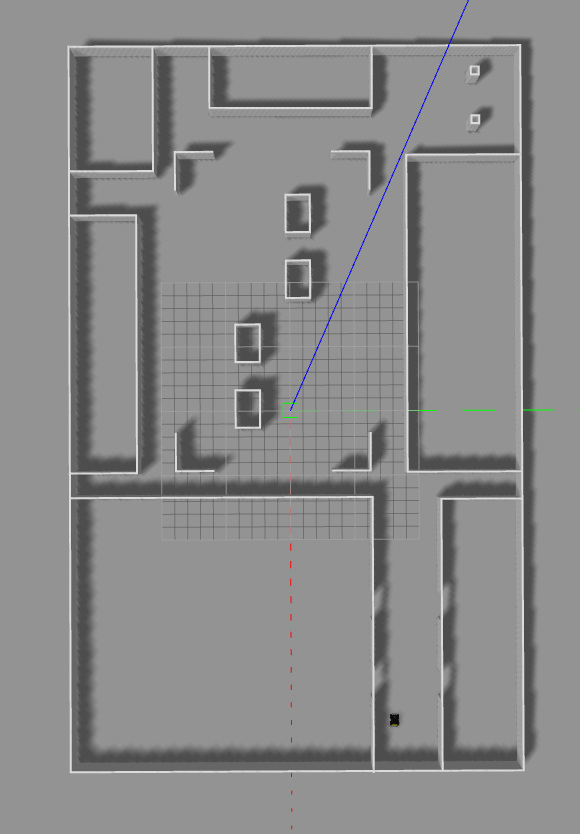
\includegraphics[width=0.7\linewidth, height=0.3\textheight]{figures/WZL}
        \caption{The environment.}
        \label{fig:env}
    \end{minipage}
 \end{figure}

In order to compare localization points, the ideal trajectory has to be prepared. We decided to drive the Husky robot on a semi-rectangular open path with coordinates (0,0), (37,0), (37,13), (27,13) and (27,8) according to the $Gazebo$ world reference frame. The reason for this is that we want our robot to move through boxes elements that are centered in the environment, like in Figure \ref{fig:env}. Performing such sharp movements in such narrow spaces resambles a robot approaching and passing through production line sites. \\
The $ideal$ path has been created making an own node called $using-markers$ in Rviz. Markers [4] are special types of visualization objects that serve for this purpose. We decided to leave the Global planner strategy from previous updates [3], since lacking of flexibility and accuracy for this big environment. The Rviz markers are seen in Figure \ref{fig:markers}.

 \begin{figure}[h]
	\center
	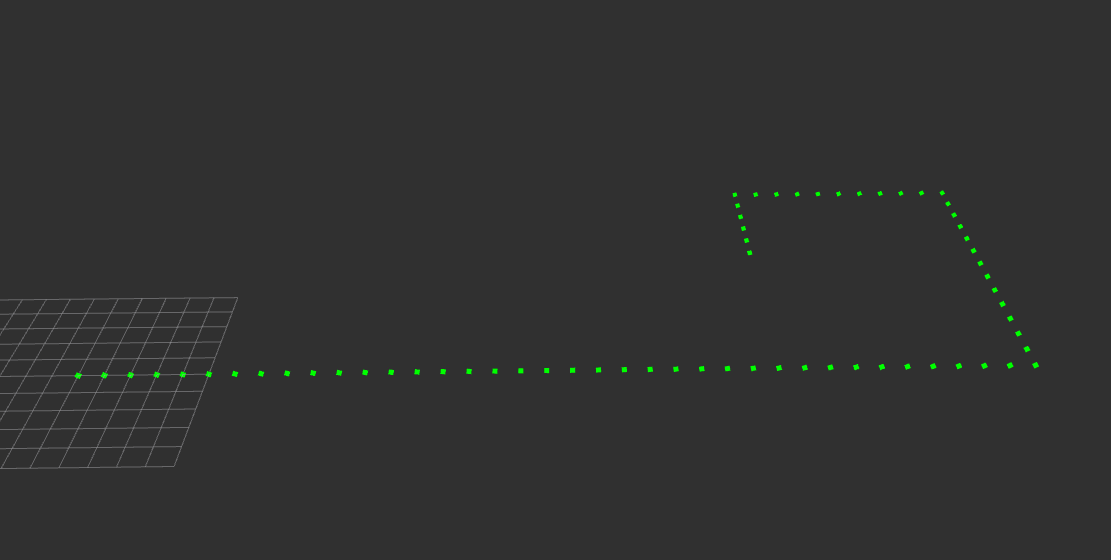
\includegraphics[width=1\textwidth]{figures/globalreference_path.png}
	\caption{Rviz markers are seen as little green rectangles and spawn one every meter. This served as the reference trajectory when registering data to be use for the successive localization}
	\label{fig:markers}
\end{figure}

The results for the 4 localization cases according to the schema of Figure \ref{fig:schema} are shown below in Figure \ref{fig:fig1}, \ref{fig:fig2}, \ref{fig:fig3}, \ref{fig:fig4}. \\
Those preliminary results are already very satisfying; red localization points do not diverge substantially from the ground thruth path in green, hence the robot`s pose can be said to be quite accurate. Nevertheless, between different mappers and localizers (cross checking them), there are already visible differences to be explained. Additionally, the data have been generated using defaults sets for both Amcl and Graph-localizer. As a next to do there is infact the tuning of the localizers parameters, as explained in the paper [5]. Afterwards we would like to have even better poses. 

\begin{figure}[H]
	\center
	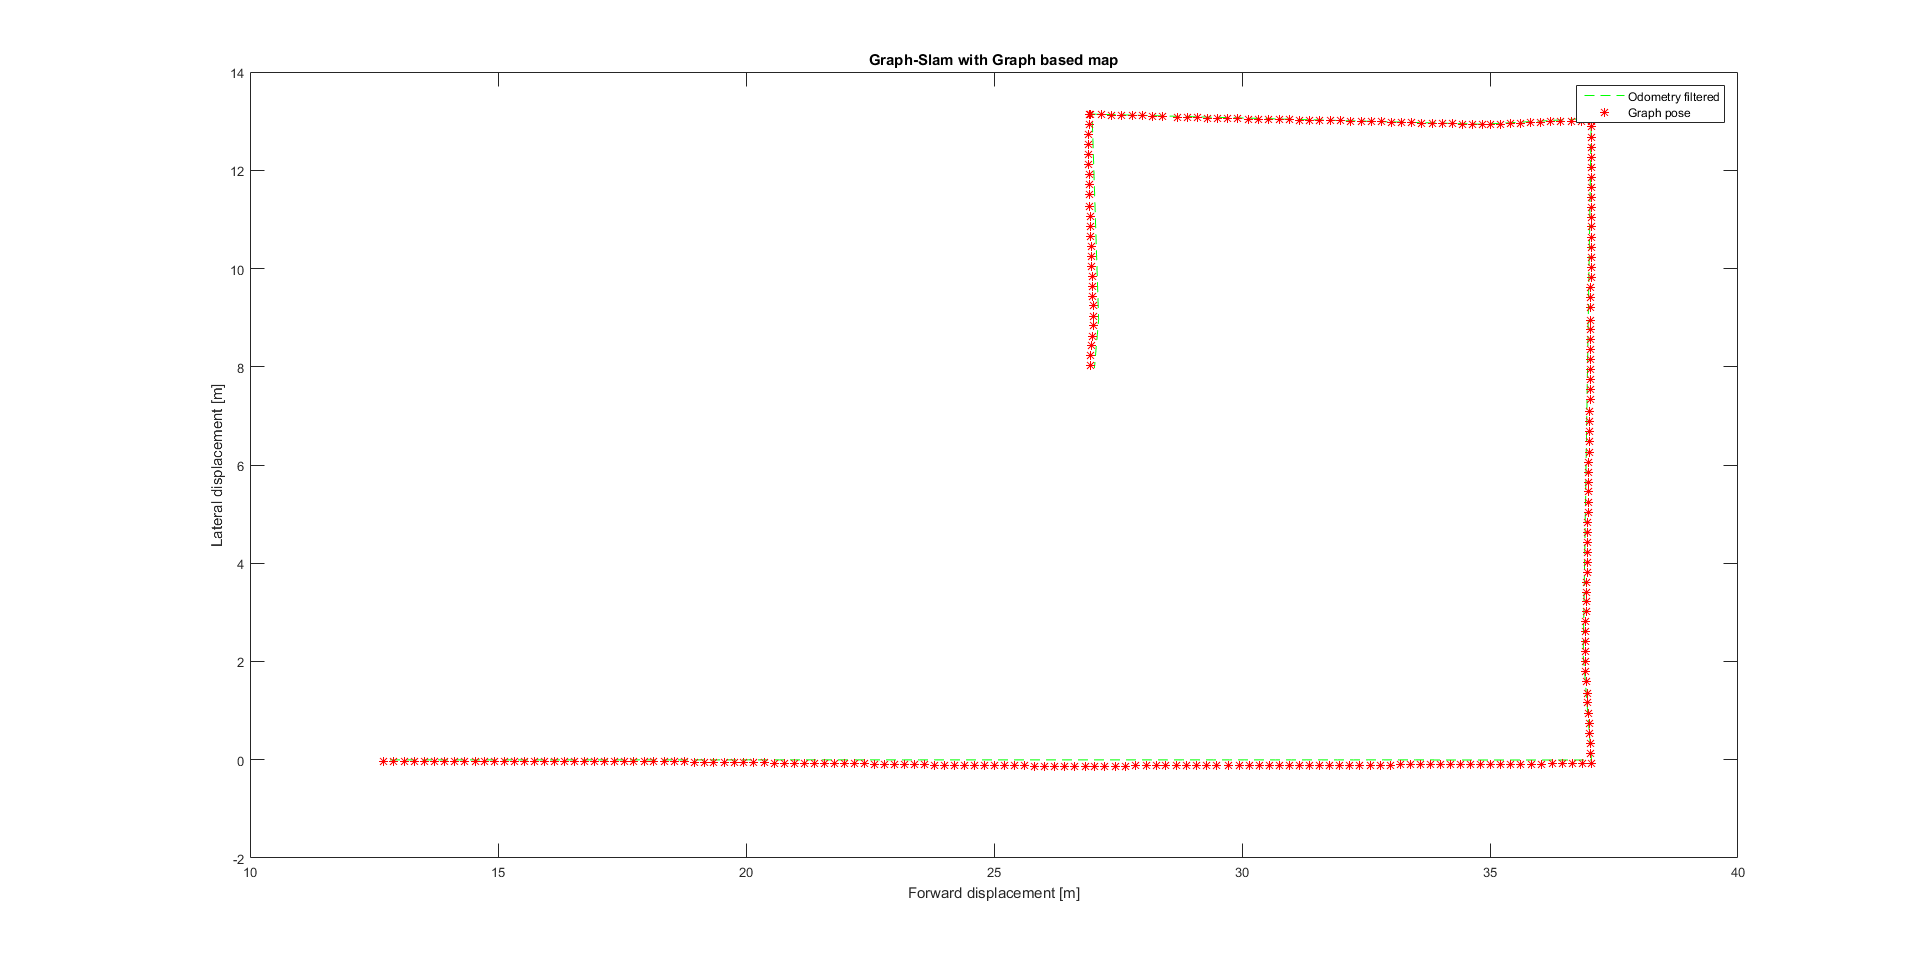
\includegraphics[width=1\textwidth]{figures/Fig1.png}
	\caption{Graph localizer with Karto-slam}
	\label{fig:fig1}
\end{figure}

\begin{figure}[H]
	\center
	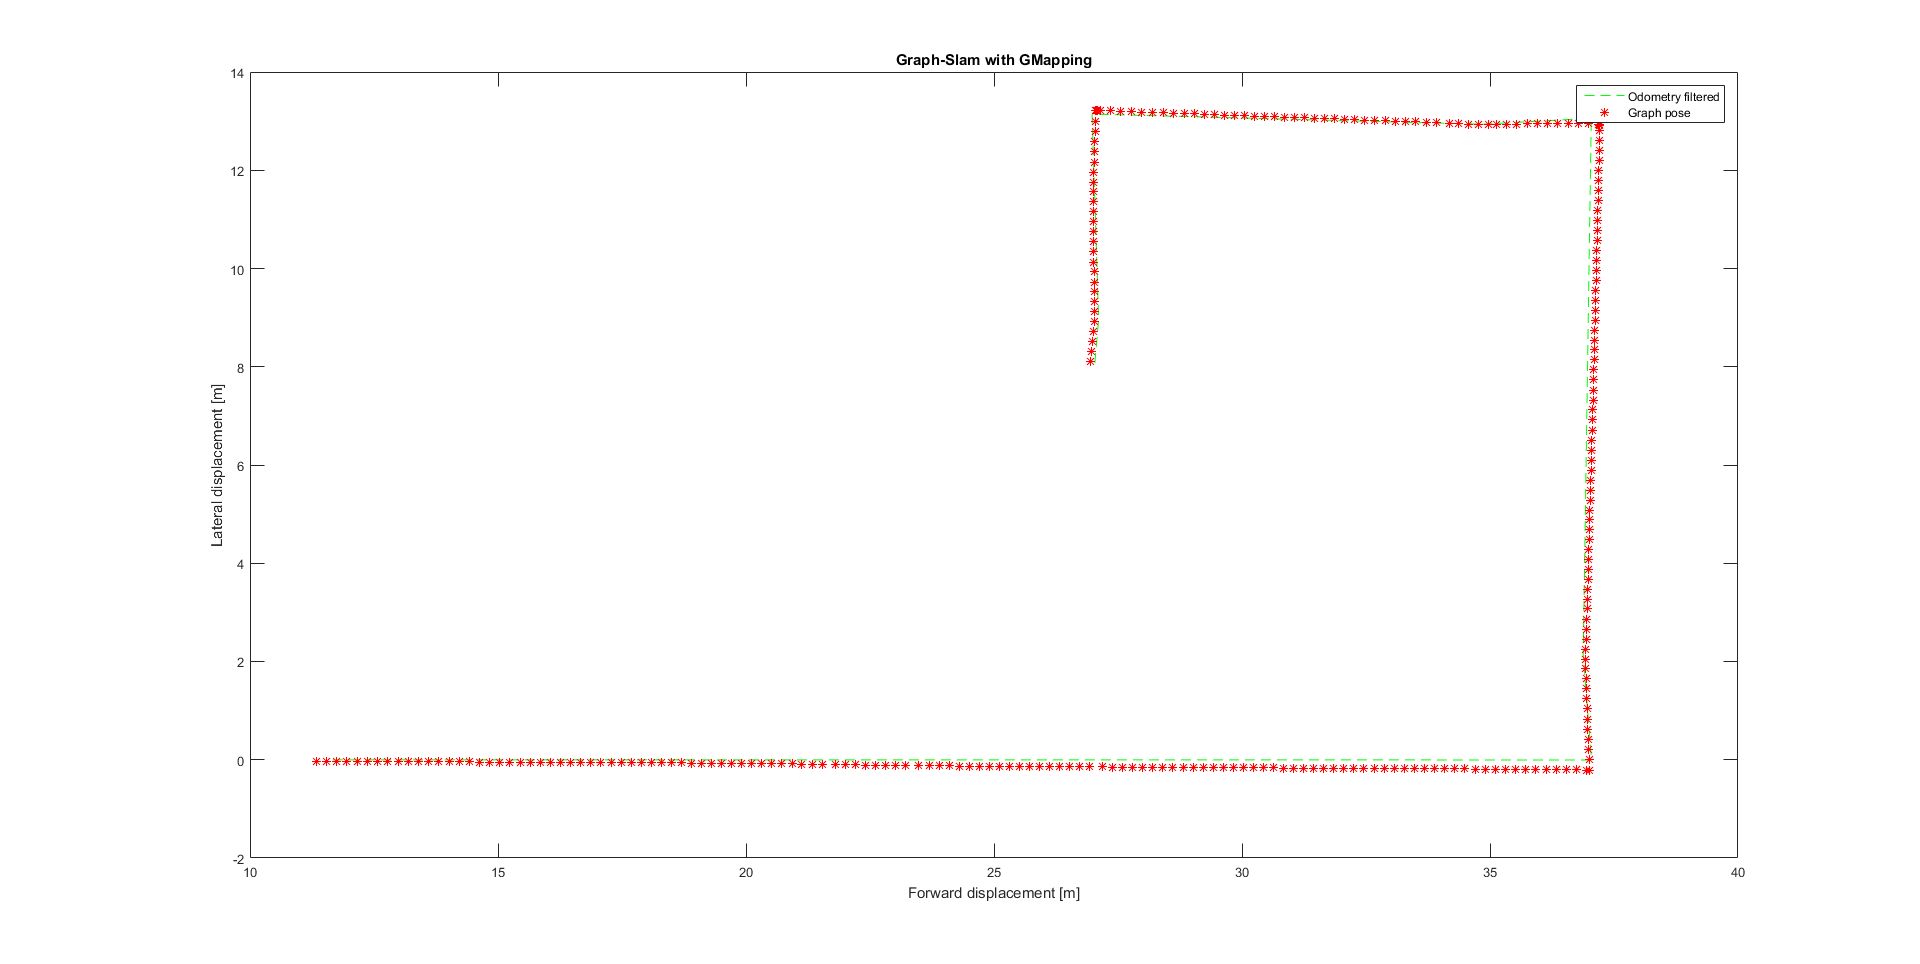
\includegraphics[width=1\textwidth]{figures/Fig2.png}
	\caption{Graph localizer with GMapping}
	\label{fig:fig2}
\end{figure}

\begin{figure}[H]
	\center
	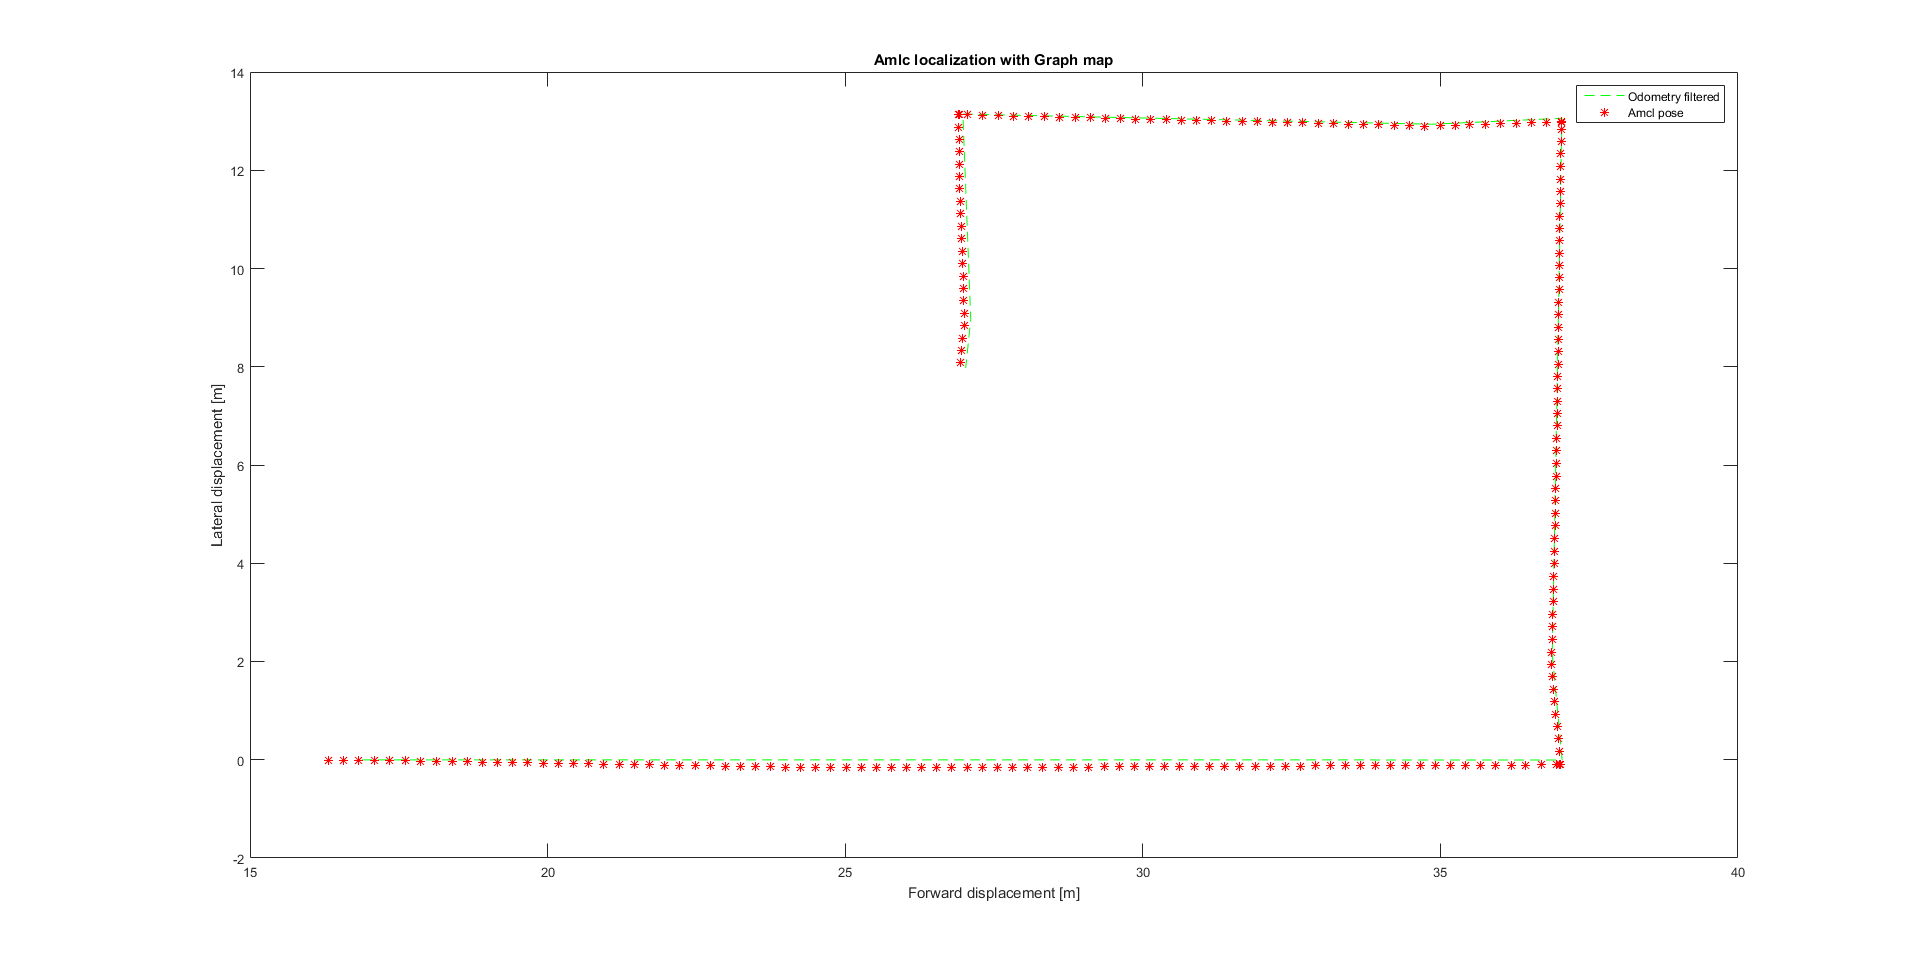
\includegraphics[width=1\textwidth]{figures/Fig3.png}
	\caption{Amcl localizer with Karto-slam}
	\label{fig:fig3}
\end{figure}

\begin{figure}[H]
	\center
	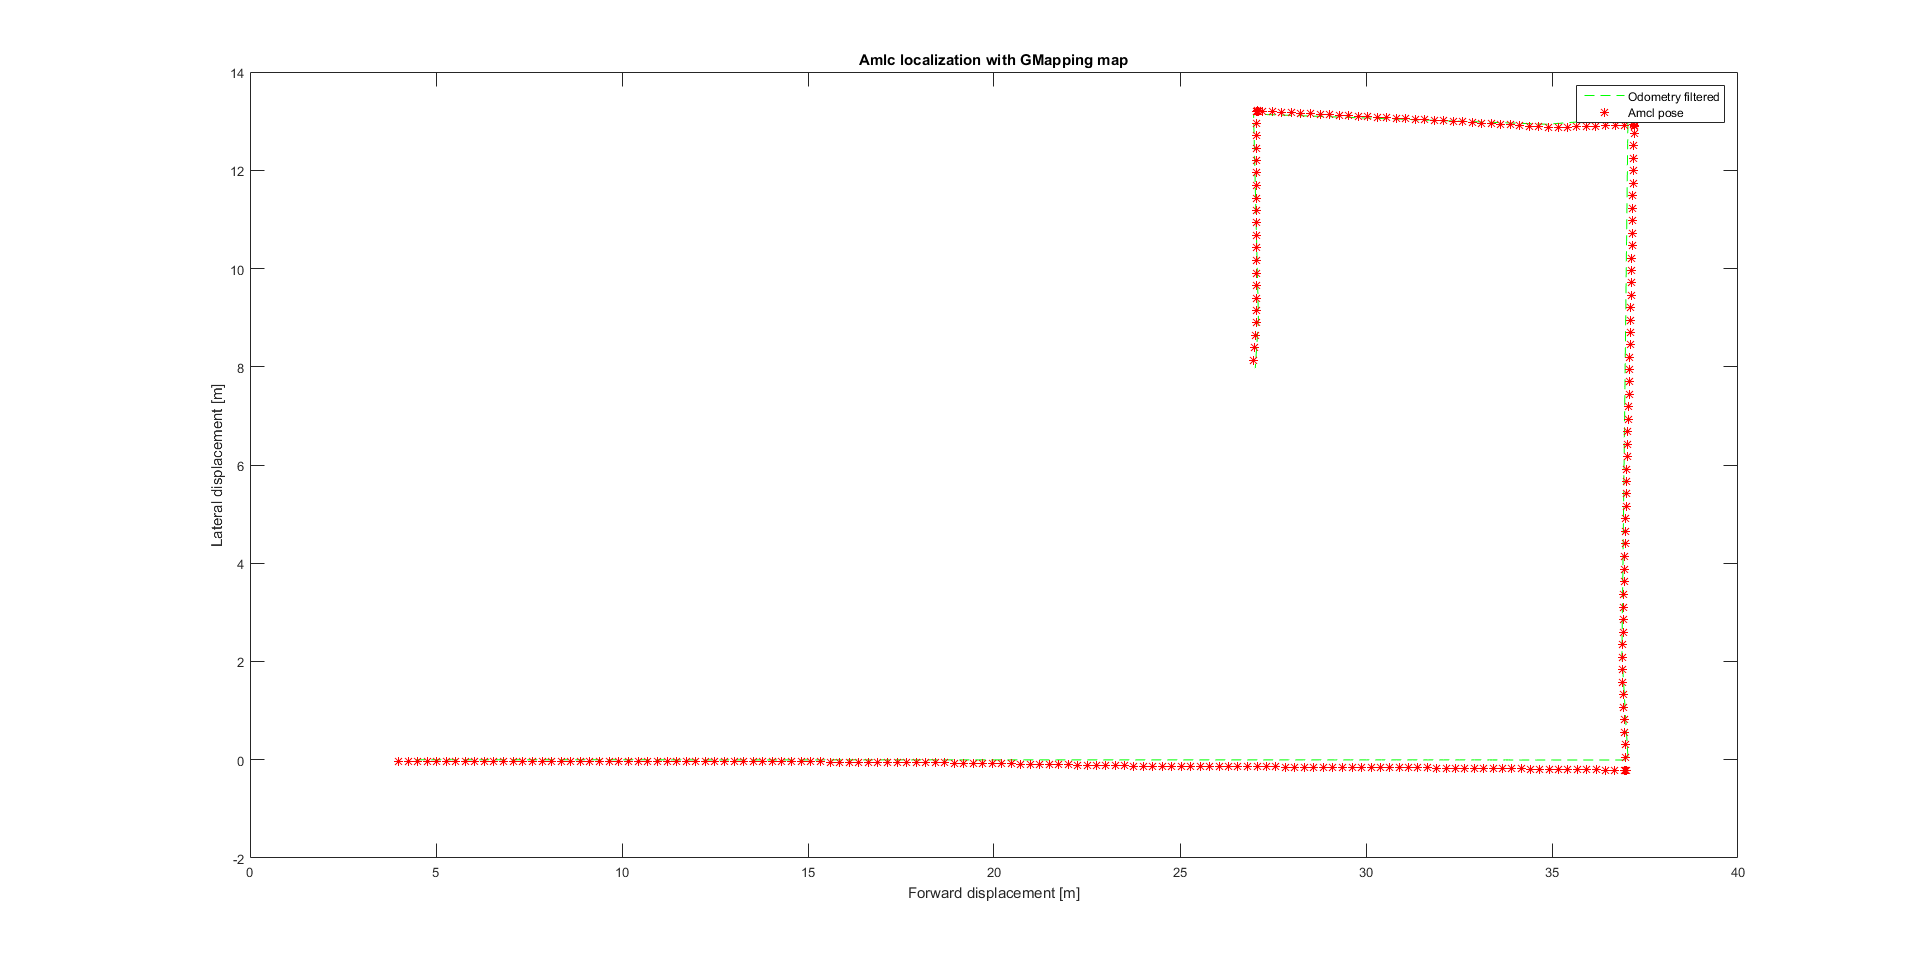
\includegraphics[width=1\textwidth]{figures/Fig4.png}
	\caption{Amcl localizer with GMapping}
	\label{fig:fig4}
\end{figure}


\section{Parameters} \label{sec:par}

As said is Section \ref{sec:comp}, default preliminary params have been adopted. Nevertherless, just $particles$ numbers have been changed, to allow the filter for rapid convergence. In Table \ref{tab:tab1} parameters for the 4 cases are summarised:

\begin{center}
\captionof{table}{Default parameters for mappers/localizers and in bold the modified ones} \label{tab:tab1}
\begin{tabular}{| m{8em} | m{13em}| m{13em}| m{9em}|} 
\hline
\textbf{GMapping} & & &\\
\hline
& \textbf{particle=50} & resampleThreshold=0,5 & LaserRange=30m\\
\hline
\textbf{Karto-slam} & & &\\
\hline
&\textbf{minparticles=100} & \textbf{maxparticles=500} &\\
\hline
\textbf{Amcl} & & &\\
\hline
&\textbf{minparticles=6000} &\textbf{maxparticles=9000} & Gmapping map\\
\hline
&\textbf{minparticles=10000} & \textbf{minparticles=15000} & Graph-map\\
\hline
\textbf{Graph-localizer} & & &\\
\hline
&\textbf{minparticles=5000} & \textbf{maxparticles=20000} & Graph-map\\
\hline
&\textbf{minparticles=10000} & \textbf{maxparticles=20000} & Gmapping-map\\
\hline
\end{tabular}
\end{center}

\section{What is next}

The third and last localization method with the use of remote signals tags. According to my recent researches this will be with the use of RFID tags or QR code camera based localization.



\section{References} \label{sec:ref}
[1]: http://wiki.ros.org/nav2d
[2]: An Evaluation of 2D SLAM Techniques Available in ROS
[3]: Update document 20/11/2017
[4]: http://wiki.ros.org/interactive{\_}markers
[5]: Robotic exploration for mapping and change detection, Sebastian Gangl

\end{document}



% == TABLE ==
%begin{table}[h!]
 % \centering
  %\caption{Caption for the table.}
 % \label{tab:table1}
 % \begin{tabular}{ccc}
 %   \toprule
  %  Some & actual & content\\
   % \midrule
   % prettifies & the & content\\
   % as & well & as\\
  %  using & the & booktabs package\\
  %   \bottomrule
  %\end{tabular}
%\end{table}


% === ALGORITHM == 


\iffalse % multi-comment tool
\begin{algorithm}[!h]
   \caption{Kirsch, Rohig algorithm}
    \begin{algorithmic}[1]
    	\State $St-1 = St$
        \For{$i = 1$ to $N$} \Comment{With N the number of particles in the filter set by maxparticle parameter}
            \State $Spread $ $particles$ $in$ $the$ $anchorbox$ $with$ $equations$ $1)$ $and$ $2)$ $of$ $[3]$ \Comment{This step is called $Global$ $Localization$}
            
            \State $xt[n] = p(xt|xt-1,ut)$ \Comment{Motion update - sample the particles from the motion update of the robot and move forward to estimate the error model functions}
            
        	\State $wt[n] = p(dnanoLOC|si)*p(dlaser|si)$ \Comment{Measurement update - si are the particles set with i the i-th index}
        	\State $St = St + <xt,wt>$ \Comment{add the state and weight to the total state space}
        	
        	\State $Perform$ $resampling$
        \EndFor
    \State $Return$ $St$

\end{algorithmic}
\end{algorithm}
\fi


\iffalse

\begin{figure}[!htb]
    \centering
    \begin{minipage}{.5\textwidth}
        \centering
        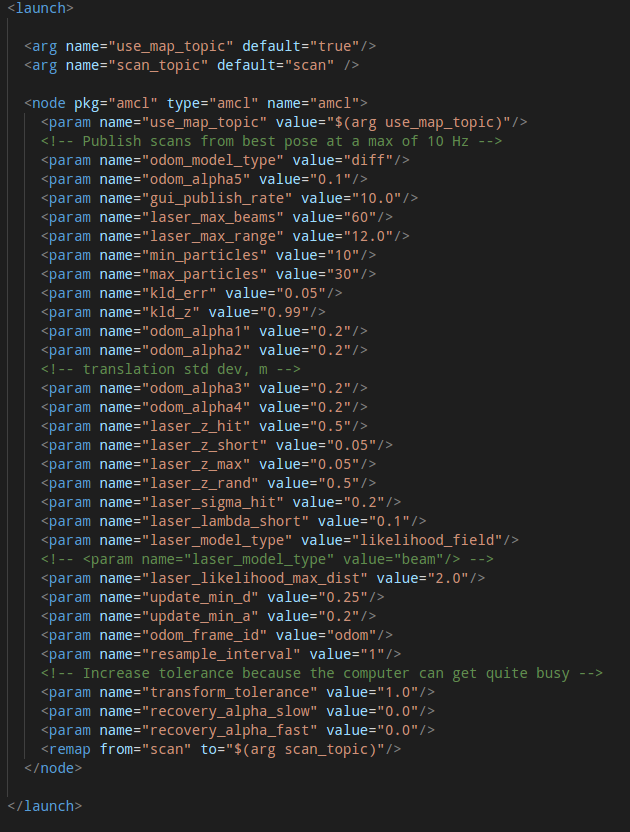
\includegraphics[width=0.7\linewidth, height=0.2\textheight]{figures/amcl_param}
        \caption{The $amcl$ tunable parameters}
        \label{fig:amcl_param}
    \end{minipage}%
    \begin{minipage}{0.5\textwidth}
        \centering
        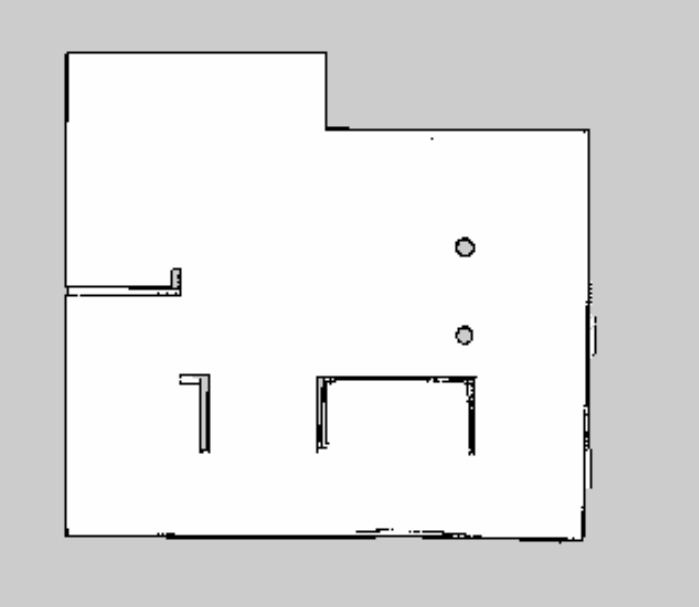
\includegraphics[width=0.7\linewidth, height=0.2\textheight]{figures/my_amcl_gmapping}
        \caption{Result of the Gmapping for the simple indoor environment}
        \label{fig:myamcl_map}
    \end{minipage}
 \end{figure}

% 3 column figure

{\_}




\begin{figure}[h]
\minipage{0.32\textwidth}
  \includegraphics[width=\linewidth]{figures/goal.png}
  \caption{The planner is tested by setting an arbitrary goal in the environment; this shouldn't coincise with the last point of the Planner. No matter where it is set, the robot sticks to the Planner path as soon as the goal is reached}\label{fig:goal}
\endminipage\hfill
\minipage{0.32\textwidth}
  \includegraphics[width=\linewidth]{figures/start.png}
  \caption{The Planner path (pink) is drawn, particles are initialized and the robot starts to move}\label{fig:start}
\endminipage\hfill
\minipage{0.32\textwidth}%
  \includegraphics[width=\linewidth]{figures/end.png}
  \caption{The robot reaches the goal}\label{fig:end}
\endminipage
\end{figure}

 
 
 \begin{figure}[!htb]
	\center
	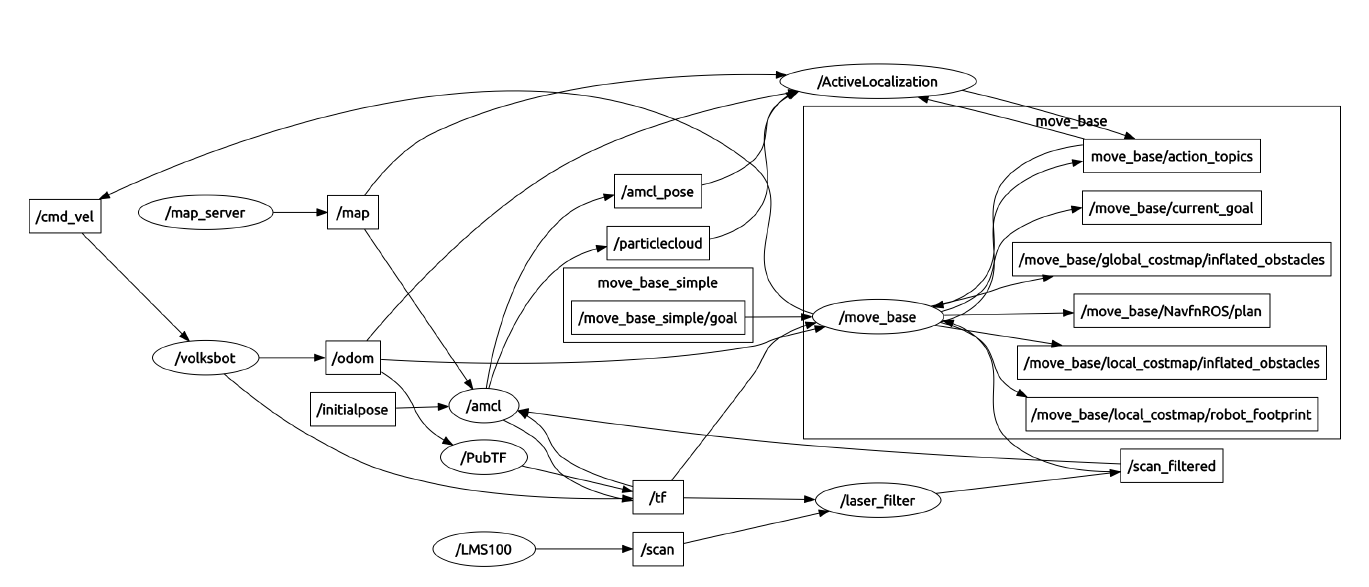
\includegraphics[width=1\textwidth]{figures/active_localization_node.png}
	\caption{An example of an active localization node}
	\label{fig:active_locnode}
\end{figure}

\begin{center}
\captionof{table}{GMapping default parameters} \label{tab:Table3}
\begin{tabular}{| m{12em} | m{13em}|} 
\hline
\textbf{Particles} & \textbf{ResThreshold} \\
\hline
particle=5 & Thr=0.1\\
\hline
particle=50 & Thr=1\\
\hline
particle=5 & Thr=1\\
\hline
particle=50 & Thr=0.1 \\
\hline
\end{tabular}
\end{center}

% underscore symbol {\_}


\fi